% !TeX document-id = {0be8c18c-9430-4e9a-bdd9-12beadebfebc}
% !TeX TXS-program:bibliography = txs:///biber
\documentclass[11pt]{beamer}
\uselanguage{portuguese}
\languagepath{portuguese}
\deftranslation[to=portuguese]{Theorem}{Teorema}
\deftranslation[to=portuguese]{theorem}{teorema}
\deftranslation[to=portuguese]{Example}{Exemplo}
\deftranslation[to=portuguese]{example}{exemplo}
\deftranslation[to=portuguese]{Lemma}{Lema}
\deftranslation[to=portuguese]{lemma}{Lema}
\deftranslation[to=portuguese]{Corollary}{Corolário}
\deftranslation[to=portuguese]{corollary}{corolário}
%\deftranslation[to=portuguese]{and}{e}

\usepackage[brazilian]{babel}
\usepackage[utf8]{inputenc}
\usepackage[T1]{fontenc}
\usepackage{lmodern}
\usepackage{amsmath}
\usepackage{amssymb}
\usepackage{mathtools}
\usepackage{color}
\usepackage{pgfplots}
\usepackage{tikz}

%\usepackage{appendixnumberbeamer}

\newenvironment{transitionframe}{
	\setbeamercolor{background canvas}{bg=yellow}
	\begin{frame}}{
	\end{frame}
}
\usetheme{default}
\usefonttheme{structuresmallcapsserif}

%% I use a beige off white for my background
\definecolor{MyBackground}{RGB}{255,253,218}
\useinnertheme[shadow]{rounded}
\setbeamercolor{block title}{bg=MyBackground}
\setbeamercolor{block body}{bg=MyBackground}
\setbeamercolor{example title}{bg=MyBackground}
\setbeamercolor{example body}{bg=MyBackground}


\newcommand{\blue}[1]{\textcolor{blue}{#1}}
\newcommand{\red}[1]{\textcolor{red}{#1}}
\newcommand{\purple}[1]{\textcolor{purple}{#1}}
\newcommand{\gray}[1]{\textcolor{gray}{#1}}
\setbeamertemplate{navigation symbols}{}
%\setbeamertemplate{page number in head/foot}[appendixframenumber]

%\usepackage{graphics}
\usepackage{graphicx}

\definecolor{blue_emph}{RGB}{0,114,178}
\definecolor{red}{RGB}{213,94,0}
\definecolor{yellow}{RGB}{240,228,66}
\definecolor{green}{RGB}{0,158,115}
\definecolor{purple}{RGB}{204,121,167}
\definecolor{orange}{RGB}{230,159,0}
\definecolor{lightblue}{RGB}{86,180,233}

%\setbeamercolor{frametitle}{fg=blue}
%\setbeamercolor{title}{fg=blue}
\setbeamertemplate{footline}[frame number]
\setbeamertemplate{navigation symbols}{} 
\setbeamertemplate{itemize items}{-}
%\setbeamercolor{itemize item}{fg=blue}
%\setbeamercolor{itemize subitem}{fg=blue}
\setbeamertemplate{enumerate items}[default]
%\setbeamercolor{enumerate subitem}{fg=blue}
\setbeamercolor{button}{bg=MyBackground,fg=blue}
\usefonttheme{structuresmallcapsserif}

%\setbeamercolor{section in toc}{fg=blue}
%\setbeamercolor{subsection in toc}{fg=red}
\setbeamersize{text margin left=1em,text margin right=1em} 


\usepackage{appendixnumberbeamer}

\usepackage[
backend=biber,
style=authoryear,
natbib=true
]{biblatex}
\addbibresource{../bibliography.bib}

\newenvironment{wideitemize}{\itemize\addtolength{\itemsep}{10pt}}{\enditemize}
\newenvironment{wideenumerate}{\enumerate\addtolength{\itemsep}{10pt}}{\endenumerate}
\newenvironment{halfwideitemize}{\itemize\addtolength{\itemsep}{0.5em}}{\enditemize}
\newenvironment{halfwideenumerate}{\enumerate\addtolength{\itemsep}{0.5em}}{\endenumerate}


\author{Luis A. F. Alvarez}
\title{EAE1223: Econometria III}
\subtitle{Aula 2 - Processos estocásticos}
%\logo{}
%\institute{}
\date{\today}
%\subject{}
%\setbeamercovered{transparent}

\begin{document}

	\begin{frame}[plain]
	\maketitle
	\end{frame}
	\begin{frame}{Espaço de probabilidade}
		\begin{itemize}
			\item Formalmente, o conceito utilizado para se definir a noção de incerteza associada a um problema é o de {\color{blue}espaço de probabilidade}.
			\item Um espaço de probabilidade é uma tripla $(\Omega, \Sigma, \mathbb{P})$, onde:
			\begin{itemize}
				\item $\Omega$ é um conjunto, denominado {\color{blue}espaço amostral}, contendo todos as possíveis realizações da incerteza.
				\item $\Sigma$ é uma coleção de subconjuntos de $\Omega$, denominada {\color{blue}$\sigma$-álgebra}. A cada subconjunto de $\Omega$ pertencente a $\Sigma$  damos o nome de {\color{blue}evento}. Os elementos de $\Sigma$ são aqueles para os quais somos capazes de definir a incerteza.
				\item uma {\color{blue}lei de probabilidade} $\mathbb{P}$ que atribui, a cada conjunto $E \in \Sigma$, um número $\mathbb{P}[E]$ entre $0$ e $1$. A lei de probabilidade satisfaz os {\color{blue}axiomas de Kolmogorov}.
			\end{itemize}
			\item Por que não definimos a probabilidade para todo subconjunto de $\Omega$?
			\begin{halfwideitemize}
				\item \textbf{Resposta:} se $\Omega$ é ``complexo'' (por exemplo, $[0,1]$), é impossível definir uma probabilidade que satisfaça todos os axiomas de Kolmogorov para todo subconjunto do espaço.
			\end{halfwideitemize}
		\end{itemize}
	\end{frame}
	
	\begin{frame}{Exemplo}
		\begin{halfwideitemize}
			\item Considere um lançamento de um dado não viciado.
			\item Nesse caso, espaço amostral é $\Omega = \{1,2,3,4,5,6\}$.
			\item Como lançamento é não viciado, sabemos que:
			$$\mathbb{P}[\{1\}]= \mathbb{P}[\{2\}] = \mathbb{P}[\{3\}] = \mathbb{P}[\{4\}] = \mathbb{P}[\{5\}] = \mathbb{P}[\{6\}] = 1/6 \,.$$
			\item Pelos axiomas da probabilidade, segue que podemos tomar $\Sigma$ como o conjunto de todos os subconjuntos de $\Omega$, e, para qualquer $E\subset \Sigma$:
			$$\mathbb{P}[E]= \mathbb{P}[\cup_{e \in E}\{e\}] = \sum_{e \in E}\mathbb{P}[\{e\}] = \frac{\# E}{6}\, ,$$
			onde $\# E$ é o número de elementos de $E$.
			\item Exemplo: probabilidade de que o lançamento dê um número par é:
			$$\mathbb{P}[\{2,4,6\}]= \frac{3}{6} = \frac{1}{2}$$
		\end{halfwideitemize}
	\end{frame}
	
	
	\begin{frame}{Variável aleatória e processo estocástico}
		\begin{halfwideitemize}
			\item Uma {\color{blue}variável aleatória} $Z$ é uma {\color{blue}função}, com domínio no espaço amostral (onde definimos a incerteza), e valores em outro espaço (para nossos fins, os reais).
			\begin{itemize}
				\item Por exemplo, $(\Omega, \Sigma, \mathbb{P})$ um espaço de probabilidade descrevendo a incerteza associada aos retornos de ativos financeiros, e $Z: \Omega \mapsto \mathbb{R}$ é a variável aleatória que representa o retorno de um fundo.
				\item Incerteza em $(\Omega, \Sigma, \mathbb{P})$ traduz-se em incerteza em $Z$, i.e. $Z$ é incerto pois o valor $\omega \in \Omega$ que ocorre é incerto.
			\end{itemize}
			\item Um {\color{blue} processo estocástico} é uma coleção de variáveis aleatórias $\{X_t: t \in \mathcal{T}\}$, com domínio no \textbf{mesmo} espaço de probabilidade e indexada por um conjunto $\mathcal{T}$
			\item Uma {\color{blue}série de tempo} é um processo estocástico indexado no tempo, i.e. $\mathcal{T}$ é um conjunto de períodos.
			\begin{halfwideitemize}
				\item Sempre tomaremos $\mathcal{T} = \mathbb{Z}$ ou $\mathcal{T}  =\mathbb{N}$.
				\item Para cada $\omega \in \Omega$, $\{ X_t(\omega): t \in \mathcal{T} \}$ é uma trajetória {\color{blue}possível} da série de tempo. Para cada $t \in \mathcal{T}$, $X_t$ é uma variável aleatória.
			\end{halfwideitemize}
		\end{halfwideitemize}
	\end{frame}
	
	\begin{frame}{Série de tempo estritamente estacionária}
		\begin{itemize}
			\item Uma série de tempo $\{X_t: t \in \mathcal{T}\}$ é dita estritamente estacionária se, para todo $t \in \mathcal{T}$, $j\in \mathbb{N}$:
			
			$$(X_t, X_{t+1}, \ldots, X_{t+j}) \overset{d}{=} (X_{t+h}, X_{t+1+h}, \ldots, X_{t+j+h})\,, \quad \forall h \geq 0 \, , $$
			onde $\overset{d}{=}$ significa igualdade das distribuições conjuntas, isto é
			
			\begin{align*}
				\mathbb{P}[X_t \leq c_1, X_{t+1} \leq c_2, \ldots, X_{t+j} \leq c_j ] = \\ \mathbb{P}[X_{t+h} \leq c_1, X_{t+1+h} \leq c_2, \ldots, X_{t+j+h} \leq c_j ], \quad \forall c_1,c_2\ldots, c_j \, .
			\end{align*}
			
			\item Estacionariedade estrita requer que distribuição de qualquer número finito de períodos do processo seja a mesma ao longo do tempo.
		\end{itemize}
	\end{frame}
	
		\begin{frame}{Série de tempo fracamente estacionária}
			
			\begin{itemize}
				\item Para modelos lineares de séries de tempo, vamos considerar o conceito de {\color{blue}processo (fracamente) estacionário}.
				\item Uma série de tempo $\{X_t: t \in \mathcal{T}\}$ é dita {\color{blue}(fracamente) estacionária} se:
				\begin{halfwideenumerate}
					\item $\mathbb{E}[X_{t}] = \mu$ para todo $t \in \mathcal{T}$.
					\item $\mathbb{V}[X_{t}] = \sigma^2 < \infty$ para todo $t \in \mathcal{T}$.
					\item $\text{cov}(X_t, X_s) = \phi_{|t-s|}$ para todo $t,s \in \mathcal{T}$.
				\end{halfwideenumerate}
				\item Processo é fracamente estacionário se sua média e variância mantêm-se constantes no tempo e covariância entre duas observações depende somente da distância entre as duas observações no tempo.
				\item Estacionariedade fraca impõe um {\color{blue}mínimo} de estabilidade no processo ao longo do tempo para que análise estatística usual possa prosseguir.
				\begin{itemize}  
					\vspace{-1em}
					\item De modo geral, alguma noção de estacionariedade + dependência fraca entre as observações (observações muito distantes no tempo comportam-se ``como'' observações independentes) vai ser requerida das séries de tempo para o funcionamento ``padrão'' de estimadores.
				\end{itemize}
				\item Processo é dito {\color{blue}não estacionário} se não for fracamente estacionário.
			\end{itemize}

	\end{frame}
	

	
	\begin{frame}{Ruído branco}
	\begin{wideitemize}
		\item Um processo $Z_t$, $t \in \mathcal{T}$, é dito um {\color{blue}ruído branco} se:
		\begin{halfwideenumerate}
			\item $\mathbb{E}[Z_t] = 0$ para todo $t$.
			\item $\mathbb{V}[Z_t] = \sigma^2 < \infty$ para todo $t$.
			\item $\text{cov}(Z_t, Z_s) = 0$ se $t \neq s$.
		\end{halfwideenumerate}
		\item Um ruído branco tem média zero, variância constante finita e não apresenta correlação serial.
		\begin{halfwideitemize}
			\item Por construção, é um processo fracamente estacionário.
		\end{halfwideitemize}
	\end{wideitemize}
\end{frame}
\begin{frame}{Ruído branco (gráfico)}
	\begin{figure}
		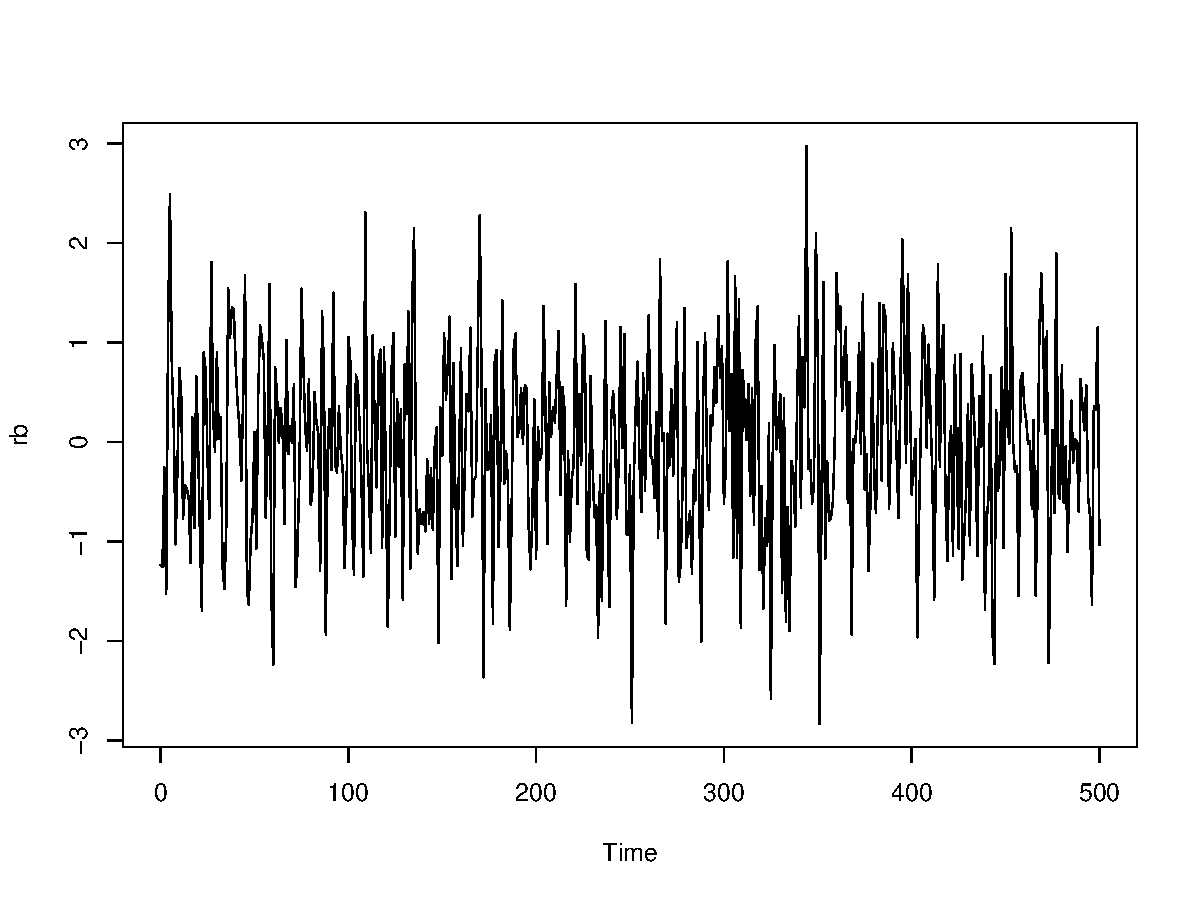
\includegraphics[scale=0.5]{graficos/rb.pdf}
	\end{figure}
\end{frame}
\begin{frame}{Processo  MA(q)}
	\begin{halfwideitemize}
			\item Um processo $Z_t$, $t \in \mathbb{Z}$, é dito de média movel de ordem $q$, ou tão somente MA(q), se:
			
			$$Z_t = \mu + \epsilon_t + \sum_{j=1}^{q} \psi_q \epsilon_{t-j} \, ,$$
			onde $\{\epsilon_t\}_t$ é um ruído branco com variância $\sigma^2_\epsilon$.
			\item Vamos verificar que o processo é (fracamente) estacionário. De fato
			\begin{enumerate}
				\item 			$\mathbb{E}[Z_t] = \mu $.
				\item $\mathbb{V}[Z_t] = \sigma^2_\epsilon(1+ \sum_{j=0}^q\psi^2_j)$.
				\item $\operatorname{cov}( Z_{t+j}, Z_t) = \begin{cases}
					\sigma^2_\epsilon (\psi_{j} + \psi_{j+1}\psi_1 + \psi_q \psi_{q-j}), & \text{se } 0 < j  \leq q \\
					0,& \text{se } j  > q
				\end{cases}$
			\end{enumerate}
			\item Processo tem memória curta: correlações desaparecem após $q$ períodos.
	\end{halfwideitemize}
\end{frame}

\begin{frame}{Processo MA(2) com $\psi_1=1$ e $\psi_2 = 0.5$}
		\begin{figure}
		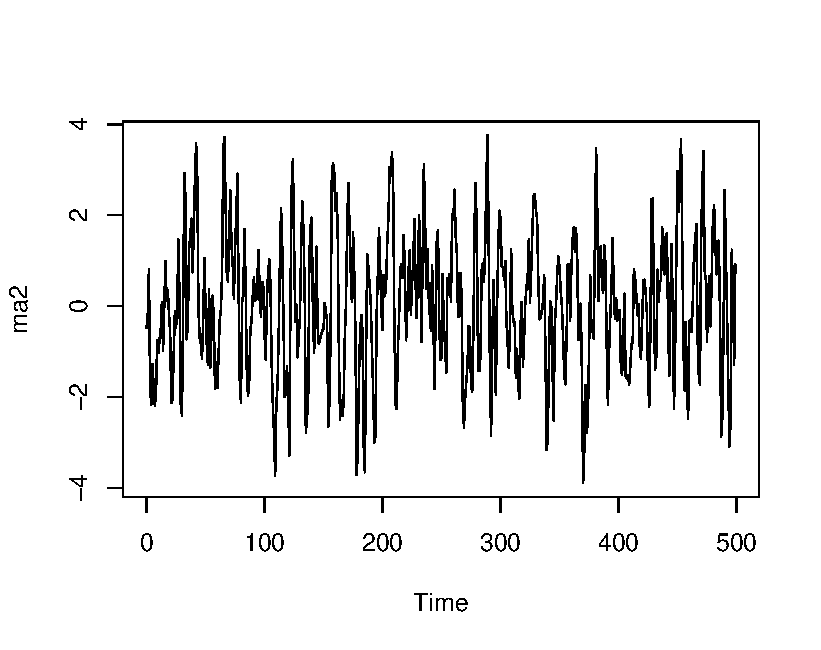
\includegraphics[scale=0.8]{graficos/ma2.pdf}
	\end{figure}
\end{frame}
\begin{frame}{Processo  AR(1) estacionário}
	\begin{wideitemize}
		\item Um processo $Z_t$, $t \in \mathbb{Z}$, é dito autorregressivo de ordem um estacionário, ou tão somente AR(1) estacionário, se:
		\begin{equation*}
			Z_t = \alpha + \rho Z_{t-1} + u_t
		\end{equation*} 
		onde $|\rho| < 1$, $\{u_t\}_{t \in \mathbb{Z}}$ é ruído branco com $\mathbb{V}[u_t] = \sigma^2_u$ existem $S \in \mathbb{Z}$, $C \in \mathbb{R}$  tais que $\mathbb{E}[|Z_t|] \leq C$ para todo $t \leq S$.
		
		\item Vamos verificar que as condições acima garantem que o processo seja, de fato, estacionário.
		\item Note que:
		
		\begin{equation*}
			\begin{aligned}			
				Z_t &=  \alpha + \rho(\alpha + \rho Z_{t-2} + u_{t-1}) + u_{t}  \\
				    &= \alpha + \rho \alpha  + \rho^2(\alpha + \rho Z_{t-3} + u_{t-2}) + u_{t} + \rho u_{t-1} \\
				     &`= \ldots \\
				     & = \sum_{j=0}^{\tau} \rho^{j} \alpha +  \rho^{\tau} Z_{t-\tau} +  \sum_{j=0}^{\tau} \rho^{j} u_t\\
			\end{aligned}
		\end{equation*}
		
		

	\end{wideitemize}
\end{frame}

\begin{frame}{Processo AR(1) estacionário (cont.)}
	\begin{halfwideitemize}
		\item Pelas hipóteses, $\lim_{\tau \to \infty} \rho^{\tau} \mathbb{E}[|Z_{t-\tau}|] = 0$. Isso nos garante que $\rho^{\tau} |Z_t| \to 0$ e podemos escrever
		
		$$Z_t = \sum_{j=0}^{\infty} \rho^{j} \alpha +   \sum_{j=0}^{\infty } \rho^{j} u_t = \frac{\alpha}{1-\rho} + \sum_{j=0}^\infty \rho^j u_{t-j}$$
		\item AR(1) estacionário se escreve como MA($\infty$).
		\item Usando representação acima, podemos checar que o processo é estacionário. De fato:
			\begin{halfwideenumerate}
			\item $\mathbb{E}[Z_t] = \frac{\alpha}{1-\rho}$
			\item $\mathbb{V}[Z_t] = \frac{\sigma^2_u}{1-\rho^2}$.
			\item $\operatorname{cor}(Z_t, Z_s) = \rho^{|t-s|}$.
		\end{halfwideenumerate}
	\end{halfwideitemize}
\end{frame}

\begin{frame}{AR(1) estacionário com $\rho = 0.7$ (gráfico)}
	\begin{figure}
		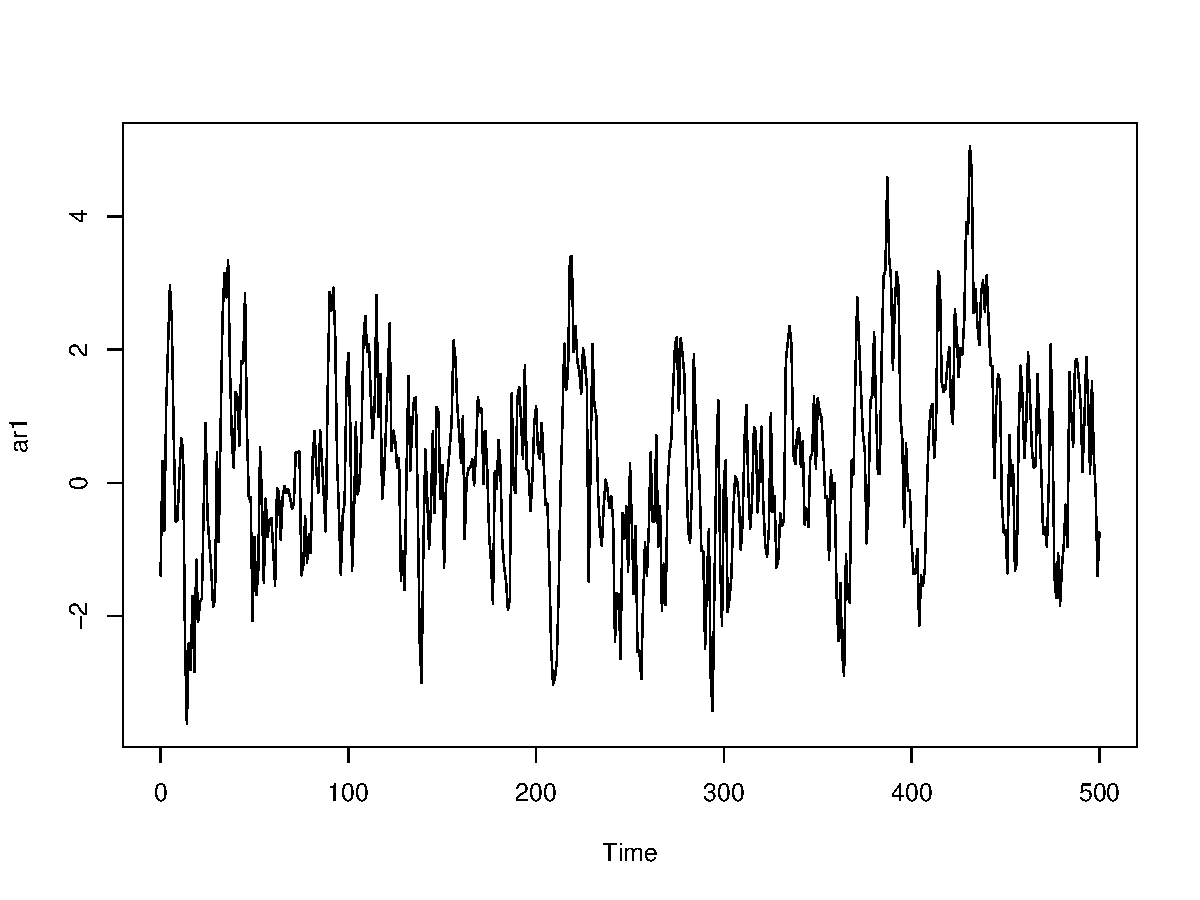
\includegraphics[scale=0.5]{graficos/ar1.pdf}
	\end{figure}
\end{frame}

	
	
		\begin{frame}{Processo AR(p) estacionário}
		\begin{halfwideitemize}
				\item Um processo $Z_t$, $t \in \mathbb{Z}$, é dito autorregressivo de ordem $p$ estacionário, ou tão somente AR(p) estacionário, se:
			\begin{equation*}
				Z_t = \alpha + \beta_1 Z_{t-1} + \beta_2 Z_{t-2}+\ldots + \beta_p Z_{t-p}+ u_t
			\end{equation*} 
			onde  $\{u_t\}_{t \in \mathbb{Z}}$ é ruído branco com $\mathbb{V}[u_t] = \sigma^2_u$, existem $S \in \mathbb{Z}$, $C \in \mathbb{R}$  tais que $\mathbb{E}[|Z_t|] \leq C$ para todo $t \leq S$, e {\color{red}os parâmetros $(\beta_1,\beta_2,\ldots, \beta_p)$ são tais que processo resultante é estacionário}.
			\item No AR(p), processo se escreve como uma combinação linear do que aconteceu nos últimos $p$ períodos, mais uma inovação.
		\end{halfwideitemize}
	\end{frame}
	
	
	\begin{frame}{Operador defasagem}
		\begin{itemize}
			\item Para a análise de séries de tempo, é conveniente definir uma função $L$, denominada operador defasagem, que, para uma dada série de tempo $(X_t)_{t \in \mathcal{T}}$, nos devolve a série de tempo que consiste em  $(X_t)_{t \in \mathcal{T}}$ defasado em um período, i.e.
			
			$$L X_t \overset{\text{definição}}{=} L(X_t) = X_{t-1}, \quad \forall t \in \mathcal{T}$$
			\item A notação $L^d$ será usada para denotar a aplicação do operador $L$ $d$ vezes em sequência, i.e.
			
			$$L^d X_t \overset{\text{definição}}{=} \underbrace{L\ldots L}_{\text{d vezes}} X_t = X_{t-d}\, , \quad \forall t \in \mathcal{T}$$
			\item Por fim, definiremos $L^0 = 1$, de modo que:
			
			$$L^0 X_t = 1 X_t = X_t\, \quad \forall t \in \mathcal{T}$$
		\end{itemize}
	\end{frame}
	
	\begin{frame}{Propriedades do operador defasagem}
		\begin{block}{Lema}
			Sejam $(X_t)_{t \in \mathcal{T}}$ e $(Y_t)_{t \in \mathcal{T}}$ duas séries de tempo, e $\alpha \in \mathbb{C}$ um número complexo. Então
			\begin{enumerate}
				\item (Linearidade) $L(X_t+\alpha Y_t) =LX_t + \alpha LY_t$.
				\item (Existência de soma infinita) Se $(X_t)_{t \in \mathcal{T}}$ é estacionário e  $|\alpha|<1$, o processo
				
				$$Z_t= \sum_{j=0}^{\infty} \alpha^j L^j X_{t} = \sum_{j=0}^{\infty} \alpha^j X_{t-j}\, ,$$
				existe e é estacionário.
				\item (Inversa) Se $(X_t)_{t \in \mathcal{T}}$ é estacionário e  $|\alpha|<1$:
				
				$$(1-\alpha L)^{-1}(X_t) = \sum_{j=0}^{\infty} \alpha^j L^j X_t$$
			\end{enumerate}
		\end{block}
	\end{frame}

	\begin{frame}{AR(p) em notação polinomial}
	\begin{itemize}
	\item Usando a notação aprendida anteriormente, podemos reescrever o AR(p) como:
	\begin{equation}
		\label{eq_sol}
		\phi(L)Z_t = \alpha + u_t \, , 
	\end{equation}
	onde $\phi(L) = 1 - \beta_1L - \beta_2 L^2 \ldots - \beta_p L^p$, e $\{u\}_{t \in \mathbb{Z}}$ é ruído branco.
	\end{itemize}
		
		\begin{block}{Proposição}
			Existe um processo $\{Z_t\}_{t \in \mathbb{Z}}$ fracamente estacionário que satisfaz \eqref{eq_sol}, se, e somente se, as $p$ raízes da equação $\phi(x) = 0$ se encontram \textbf{fora} do círculo unitário, isto é:
			$$\phi(x) = 0 \implies |x| > 1 \, .$$
			
			Neste caso, o processo fracamente estacionário que satisfaz \eqref{eq_sol} é único, e pode ser escrito como:
			
			$$Z_t = \phi^{-1}(L)(\alpha + u_t) =  \tau + \sum_{j=0}^\infty \omega_j u_{t-j}$$
		\end{block}
	\end{frame}
	
	\begin{frame}{Estacionariedade do AR(p)}
\begin{itemize}
	\item A proposição anterior nos provê uma caracterização para a existência de um $\{Z_t\}_t$ estacionário que satisfaz \eqref{eq_sol}, em termos das {\color{blue}raízes do polinômio característico} $\phi(x)$.
	\begin{halfwideitemize}
		\item Note que a proposição fala de \textbf{existência} de {\color{red}uma} solução. Por quê?
		\item Isso se deve ao fato de que também podem existir processos $\{Z_t\}_{t \in \mathbb{Z}}$ não estacionários que satisfazem \eqref{eq_sol}, mesmo quando as raízes estão todas fora do círculo.
		\begin{halfwideitemize}
			\item Mas o teorema nos diz que, se ao menos uma das raízes está \textbf{dentro} do círculo, com certeza não há nenhuma solução estacionária.
		\end{halfwideitemize}
		\item A restrição que fazíamos, na definição de AR(p), de que o passado não explodia, justamente descartava as soluções não estacionárias, garantindo que estávamos selecionando a solução estacionária.
	\end{halfwideitemize}
			\item No curso e na vida, vamos seguir como tradicionalmente feito na literatura econométrica e implicitamente \textbf{sempre} descartar as soluções não estacionárias (explosivas) que existem mesmo quando todas as raízes estão fora do círculo.
			\begin{halfwideitemize}
				\item {\color{green}Dessa forma, diremos que um AR(p) é fracamente estacionário se, e somente se, todas as raízes de $\phi(x)$ estão fora do círculo.}
			\end{halfwideitemize}
\end{itemize}
\end{frame}
\begin{frame}{Encontrando os coeficientes da representação MA($\infty$)}
	\begin{itemize}
		\item As propriedades do operador defasagem podem ser utilizadas para encontrar a representação MA($\infty$) de um AR($p$) estacionáriom.
		\item De fato, considere um AR($2$) estacionário:
		$$(1-\beta_1 L - \beta_2 L^2)y_t = \alpha + u_t$$
		\item Da fatoração de polinômios,  podemos escrever:
		$$(1-\beta_1 x - \beta_2 x^2) = \left(\frac{1}{\lambda_1}x-1\right)\left(\frac{1}{\lambda_2}x-1\right)\, ,$$
		onde $\lambda_1$ e $\lambda_2$ são as raízes de $(1- x - \beta_2 x^2) = 0$.
		\item Portanto:
		$$(1-\beta_1 L - \beta_2 L^2)y_t =   \left(1- \frac{1}{\lambda_1}L\right) \left(1-\frac{1}{\lambda_2}L\right)y_t = \alpha + u_t$$
	\end{itemize}
\end{frame}

\begin{frame}{Encontrando os coeficientes da representação MA($\infty$)}
	\begin{halfwideitemize}
		\item Mas então 
		\begin{equation}
			\begin{aligned}
				y_t = (1-\beta_1 L - \beta_2 L^2)^{-1}(\alpha + u_t) = \\ \left(1-\frac{1}{\lambda_2}L\right)^{-1}\left(1- \frac{1}{\lambda_1}L\right)^{-1}(\alpha+u_t) = \\
				 \left(\sum_{i=0}^\infty \frac{1}{\lambda_2^i} L^i\right) \left(\sum_{j=0}^\infty \frac{1}{\lambda_1^j}L^j\right)(\alpha + u_t) =\\
				 \frac{1}{(1-\lambda_1^{-1})(1-\lambda_2^{-1})}\alpha + \sum_{k=0}^\infty \omega_k u_{t-k} \end{aligned}
		\end{equation}
		onde $\omega_k$ é a soma de termos $\frac{1}{\lambda^i_1 \lambda^j_2}$ tais que $i+j=k$. 
	\end{halfwideitemize}
\end{frame}

	%\begin{frame}[allowframebreaks]{Bibliografia}
	%\printbibliography
	%\end{frame}
\end{document}